%% Pattern Recognition Letters manuscript
%% Based on the official PRL template: prletters-template-with-authorship.tex
%% (elsarticle.cls + prletters.sty, twocolumn, final, authoryear)
\documentclass[times,twocolumn,final,authoryear]{elsarticle}

%% Stylefile to load PR Letters template
\usepackage{prletters}
\usepackage{framed,multirow}

%% The amssymb package provides various useful mathematical symbols
\usepackage{amssymb}
\usepackage{latexsym}
\usepackage{amsmath}
\usepackage{graphicx}
\usepackage{booktabs}

% Following three lines are needed for this document.
% If you are not loading colors or url, then these are
% not required.
\usepackage{url}
\usepackage{xcolor}
% Scope \href's second argument so font switches (e.g. \tt for arXiv ids)
% generated by model2-names.bst do not leak into subsequent bibliography entries.
\providecommand{\href}[2]{\begingroup#2\endgroup}
\definecolor{newcolor}{rgb}{.8,.349,.1}

\journal{Pattern Recognition Letters}

\begin{document}
\thispagestyle{empty}

\begin{frontmatter}

\title{When Is a Scale Redundant? Data-Dependent Scale Redundancy and Zero-Training Pruning for Real-Time Object Detection}

\author[1]{Yuanchao \snm{Yan}\corref{cor1}}
\cortext[cor1]{Corresponding author}
\ead{yanyuanchao@gnnustc.com}
\author[1]{Xin \snm{Yan}}
\ead{yanxin@gnnustc.com}
\author[1]{Jianlong \snm{Liu}}
\ead{liujianlong@gnnustc.com}

\address[1]{Department of Artificial Intelligence and Computational Science, Science and Technology College, Gannan Normal University, Ganzhou 341000, China}

\begin{abstract}
Real-time detectors run at full capacity on every image, yet where their computation is redundant is rarely quantified. We study YOLO26n on three datasets spanning opposite object-size regimes (VOC, COCO, VisDrone) and report two findings. First, scale redundancy is dataset-dependent: removing the small-object scale P3 costs 0.010/0.032/0.101 mAP on VOC/COCO/VisDrone, whereas the large-object scale P5 costs 0.417/0.176/$\approx$0; per-scale gradient contributions track the small-object fraction, and P3 versus P5 importance reverses between 3.8\% and 24.8\% small objects (a three-point crossover near 12.6\%, not a law). Second, FLOPs $\neq$ FPS: head-level cell skipping yields no GPU speedup, and the $\sim$95\% cell redundancy is only exploitable as a mask-level oracle, not as real skipping on GPU. Where a scale is truly redundant, dropping it is a zero-training optimization: on VisDrone, P5 removal cuts FLOPs/parameters by 10.4\%/28.6\% at identical mAP and reduces single-image latency by 6\%. We also report negative results---early exit is infeasible and fine-tuning a dropped scale can hurt---as cautionary evidence for FLOPs-only efficiency claims.
\end{abstract}

\begin{keyword}
\KWD real-time object detection \sep model efficiency \sep spatial token pruning \sep early exit \sep YOLO
\end{keyword}

\end{frontmatter}

\vspace*{4pt}
\noindent\textit{Keywords:} real-time object detection, model efficiency, spatial token pruning, early exit, YOLO
\vspace*{10pt}

\section{Introduction}
As LLMs that \emph{overthink} spend tokens that do not improve the answer~\cite{wei2022chain,feng2025efficient}, real-time detectors may \emph{over-see}: they compute features the input does not need. Detectors are a clean testbed because their computation decomposes into explicit units at three granularities---grid cells (tokens), feature-pyramid scales, and model checkpoints.

Prior work leaves important gaps: token-pruning methods~\cite{rao2021dynamicvit,liang2022evit,bolya2023tome,meng2021adavit} report large FLOPs savings but target attention models and report FLOPs rather than latency; early-exit detectors~\cite{teerapittayanon2016branchynet,scholte2025eobranch,anytimeyolo2025} attach confidence branches without identifying which features can be omitted; and efficiency studies are almost always single-dataset, leaving the dataset-dependence of redundancy unexamined.

This paper conducts a cross-distribution empirical study with YOLO26n~\cite{jocher2026ultralyticsyolo26unifiedrealtime} on VOC, COCO, and VisDrone, plus a cross-architecture check with YOLO11n, asking two questions. (RQ1) Is a detection scale redundant, and is the redundant scale stable across datasets? P3 is nearly redundant on VOC but critical on VisDrone, while P5 is completely redundant on VisDrone; gradient shares track the small-object fraction, and the P3/P5 ranking reverses between 3.8\% and 24.8\% small objects. (RQ2) Can redundancy become real speed? Cell-level redundancy is large (about 95\% of grid cells) but, on GPU, only exploitable as a mask-level oracle---real block skipping neither speeds up inference nor preserves accuracy without re-training. Dropping a redundant scale is instead a zero-training, latency-reducing optimization compared against input-resolution scaling and a smaller model.

Contributions: (1) a cross-distribution per-scale contribution analysis showing the redundant scale is data-dependent and tracked by the small-object fraction, with a three-point trend (not a law) reversing the P3/P5 ranking around 12.6\%; (2) an honest FLOPs-vs-FPS analysis showing cell-level redundancy is only a mask-level oracle on GPU, plus a zero-training scale-drop recipe compared against input-resolution scaling and a smaller model; (3) negative results (early exit infeasible, fine-tuning a dropped scale can hurt) as cautionary evidence.

\section{Related Work}\label{sec:related}
\emph{Dynamic token pruning and early exit.} DynamicViT~\cite{rao2021dynamicvit}, EViT~\cite{liang2022evit}, ToMe~\cite{bolya2023tome}, and AdaViT~\cite{meng2021adavit} prune or merge tokens adaptively, reporting 30--40\% FLOPs savings with negligible accuracy loss on attention models. Self-distillation of importance signals is central to TokenSkip~\cite{xia2025tokenskip} and Self-Calibration~\cite{huang2025selfcalib}. BranchyNet~\cite{teerapittayanon2016branchynet}, EOBranch~\cite{scholte2025eobranch}, and AnytimeYOLO~\cite{anytimeyolo2025} attach early-exit branches to YOLO. These lines of work share our goal---spend computation only where it helps---but report FLOPs rather than latency, target attention models or exits, and do not identify which features a detector can actually omit; for a CNN detector we show the FLOPs claim does not survive head-level cell pruning.

\emph{Dynamic computation and pruning in detectors.} Dynamic R-CNN~\cite{zhang2020dynamicrcnn} and YOLOv7~\cite{wang2023yolov7} adapt training targets or label assignment during optimization, Sparse R-CNN~\cite{sun2021sparsercnn} and Cascade RPN~\cite{vu2019cascaderpn} reduce proposal-level computation, and channel-pruning recipes---Network Slimming~\cite{liu2017networkslimming}, AutoSlim~\cite{yu2020autoslim}, and popular YOLOv5 pruning tutorials~\cite{ultralytics2023yolov5}---remove channels with negligible accuracy loss, including MCCP~\cite{yan2023mccp} for multi-collaboration channel pruning. Real-time detectors~\cite{redmon2016yolo,tian2019fcos,lin2017focal,jocher2026ultralyticsyolo26unifiedrealtime} rely on multi-scale pyramids~\cite{lin2017fpn}, and cascade~\cite{cai2018cascade} or task-aligned~\cite{feng2021tood} designs assume all scales are needed. Two differences distinguish our work. Unlike channel-pruning methods such as Network Slimming~\cite{liu2017networkslimming} or MCCP~\cite{yan2023mccp}, which find important channels by sparse training or search and then retrain, the proposed scale drop removes an entire feature-pyramid scale with zero training, because the redundant scale is identified from data statistics alone. Unlike dynamic-proposal detectors such as Sparse R-CNN~\cite{sun2021sparsercnn}, which learn a small set of object proposals, we keep the dense grid and prune the pyramid's native scales. Finally, we optimize latency (FPS) rather than FLOPs, showing where each type of saving actually transfers on GPU. On the deployment side, the cheapest generic speed-ups---reducing input resolution or removing the largest scale entirely---are common engineering practice; we treat them as first-order baselines in Sec.~4.5.
\section{Method}\label{sec:method}
\subsection{Contribution analysis}
For the FPN-style neck scales $P_3,P_4,P_5$~\cite{lin2017fpn}, the importance of scale $i$ is measured by (i) gradient contribution $G_i=\|F_i\odot\partial L/\partial F_i\|_1$ (normalized), (ii) counterfactual loss change $C_i=(L(Y^{-i})-L(Y))/L(Y)$, and (iii) detection-gain ablation $\Delta\text{AP}_i=\text{AP}(F)-\text{AP}(F_{-i})$ using a \emph{fair} head-level mask: the pruned scale produces no detections (scores $\to-\infty$), avoiding false positives from naive zero-feeding.

\subsection{Spatial token budget and self-distillation gate}
Following adaptive token pruning~\cite{rao2021dynamicvit,liang2022evit} and self-distillation of importance signals~\cite{xia2025tokenskip,huang2025selfcalib}, a gate $g_\phi$ is a per-scale $1\times1$ convolution producing cell scores; for budget $b$ we keep the top-$b$ fraction of cells per image and suppress the rest in the head. We compare an \emph{oracle} (rank by the model's own head scores), an \emph{energy} gate (rank by $\|F_i\|_1$), and a \emph{self-distilled} gate trained with the model frozen via importance-weighted BCE,
\begin{equation}
\begin{aligned}
\mathcal{L}_{\mathrm{gate}}&=\sum_i \mathrm{BCE}\big(g_\phi(P_i),t_i\big)\,w_i,\\
t_i&=\max_c\sigma(s_{i,c}),\qquad w_i=1+30t_i.
\end{aligned}
\end{equation}
where $s_{i,c}$ denotes the classification score output by the teacher's detect head (not the feature-map value) for cell $i$ and class $c$, and $t_i$ is its max-class confidence. The weight $w_i=1+30t_i$ up-weights high-confidence cells (a cell with $t_i>0.1$ receives at least $4\times$ the background weight); the gate is trained with Adam (lr $=10^{-3}$, batch 64) for 5 epochs with the backbone, neck, and head frozen.

\subsection{Zero-training scale drop}

\begin{figure*}[h]\centering
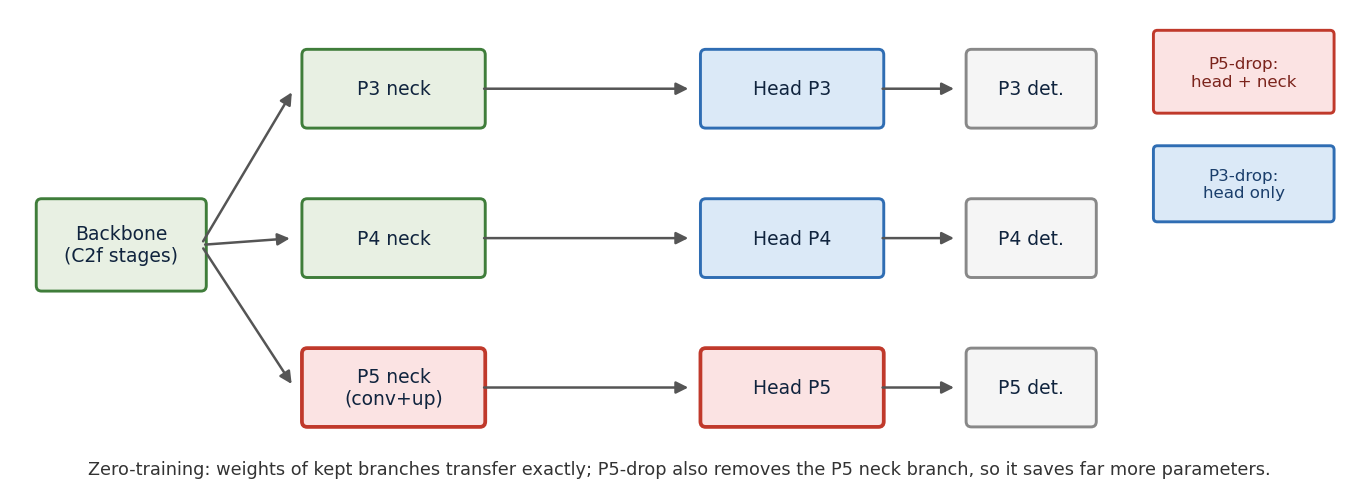
\includegraphics[width=\textwidth]{../figures/scale_drop_diagram.png}
\caption{What is dropped. P3-drop removes only the P3 branch of the detect head; P5-drop additionally removes the P5 neck branch (conv + upsampling), which is why it saves far more parameters and FLOPs.}
\label{fig:scaledrop}
\end{figure*}

Unlike conventional channel pruning, which finds important channels through retraining or search~\cite{yan2023mccp,han2015pruning}, our scale drop needs no optimization: if a scale is redundant ($\Delta\text{AP}\approx0$), it is removed and the remaining weights are transferred exactly, because removing the redundant tail branch does not change the input channels of the kept head scales. In practice we treat a scale as redundant when removal costs no more than $\approx$1\,pp of mAP50-95: P5 on VisDrone costs $\approx$0 (unambiguous), while P3 on VOC costs 1.0\,pp (0.010), a borderline case near the evaluation noise measured in Sec.~4.1. Scales costing more than 5\,pp (P5 on VOC, 0.417; P3 on VisDrone, 0.101) are clearly necessary. The 1\,pp threshold is a rule of thumb to be calibrated to the user's accuracy budget, not a certified bound.

\section{Experiments}\label{sec:exp}
\subsection{Setup}
We use YOLO26n~\cite{jocher2026ultralyticsyolo26unifiedrealtime}, initialized from COCO-pretrained weights and trained with MuSGD (batch 32, image size 640, AMP) for 100 epochs on VOC~\cite{everingham2010voc} (16\,551 train/4\,952 test2007) and VisDrone~\cite{zhu2022visdrone} (6\,471 train/548 val); COCO~\cite{lin2014coco} uses the official pretrained weights on val2017. Full training details are in the supplementary material. Ablations use fair head-level masks with the standard validator; FLOPs are measured on fused models at 640. Latency is single-GPU FP32 on an NVIDIA GeForce RTX 5070 (CUDA 13.2, no TensorRT); we report batch-32 throughput (FPS) and batch-1 per-image latency (ms), since the two can rank optimizations differently. Evaluation is deterministic: three repeated VOC evaluations give identical mAP50-95 (0.5899), so the small per-scale differences we report (e.g., 0.010 on P3-VOC) are measurements rather than evaluation noise; training-seed variance is not separately quantified.

\subsection{RQ1: scale importance is dataset-dependent}
\begin{table}[h]\centering\footnotesize
\caption{Per-scale importance is monotonically tied to the small-object fraction $s$: gradient contribution $G$ (cols. 3--4) and mAP cost $\Delta$AP of removing a scale (cols. 5--6). The redundant scale flips between VOC (drop P3) and VisDrone (drop P5).}
\label{tab:scales}
\resizebox{\linewidth}{!}{%
\begin{tabular}{lcccccc}
\toprule
Dataset & small obj. ($<$32px) & $G_{\mathrm{P3}}$ & $G_{\mathrm{P5}}$ & $\Delta$AP P3 & $\Delta$AP P5\\
\midrule
VOC & 3.8\% & 22\% & 39\% & 0.010 & 0.417\\
COCO & 24.8\% & 28\% & 30\% & 0.032 & 0.176\\
VisDrone & 85.9\% & \textbf{53\%} & 7\% & \textbf{0.101} & $-0.0001$\\
\bottomrule
\end{tabular}}

\end{table}
Fitting the three datasets (Fig.~\ref{fig:size}) gives $G_{\mathrm{P3}}(s)=0.494+0.094\ln s$ and $G_{\mathrm{P5}}(s)=0.096-0.098\ln s$ ($R^2=0.81/0.87$), crossing at $s^*\approx12.6\%$; the mAP cost follows $\Delta\text{AP}_{\mathrm{P3}}\approx0.10\,s^{0.73}$. With only three points these are trend descriptions, not laws: per-point residuals are 3.3/8.3/5.0\,pp for $G_{\mathrm{P3}}$ and 2.6/6.7/4.1\,pp for $G_{\mathrm{P5}}$ (VOC/COCO/VisDrone), and the crossover lies between the observed points at 3.8\% and 24.8\%, so 12.6\% is an interpolation within our range, not an observed phenomenon. The ranking (P3 least, P5 most important) is also stable across model sizes and architectures on COCO (Table~\ref{tab:robust}), so it is not a nano- or architecture-specific artifact.

\begin{table}[h]\centering\footnotesize
\caption{Per-scale importance is robust to model size and architecture on COCO val: the ranking $\Delta$AP P3 $<$ P4 $<$ P5 holds for YOLO26n/s/m and for YOLO11n, so the data-dependent scale-redundancy result is not specific to the nano model or to one architecture. $G$ values are normalized gradient contributions; $\Delta$AP uses the fair head-level mask.}
\label{tab:robust}
\resizebox{\linewidth}{!}{%
\begin{tabular}{lcccccc}
\toprule
Model & $G_{\mathrm{P3}}$ & $G_{\mathrm{P4}}$ & $G_{\mathrm{P5}}$ & $\Delta$AP P3 & $\Delta$AP P4 & $\Delta$AP P5\\
\midrule
YOLO26n & 28\% & 41\% & 30\% & 0.032 & 0.110 & 0.176\\
YOLO26s & 33\% & 40\% & 27\% & 0.045 & 0.156 & 0.216\\
YOLO26m & 32\% & 31\% & 38\% & 0.078 & 0.179 & 0.217\\
YOLO11n & 35\% & 37\% & 28\% & 0.017 & 0.052 & 0.186\\
\bottomrule
\end{tabular}}
\end{table}
The identity of the redundant scale is therefore transferable across model sizes on the same data: only the magnitude of the removal cost changes (e.g., $\Delta$AP P5 grows from 0.176 on YOLO26n to 0.216--0.217 on YOLO26s/m), while the ranking and hence the drop decision are preserved.

\begin{figure*}[h]\centering
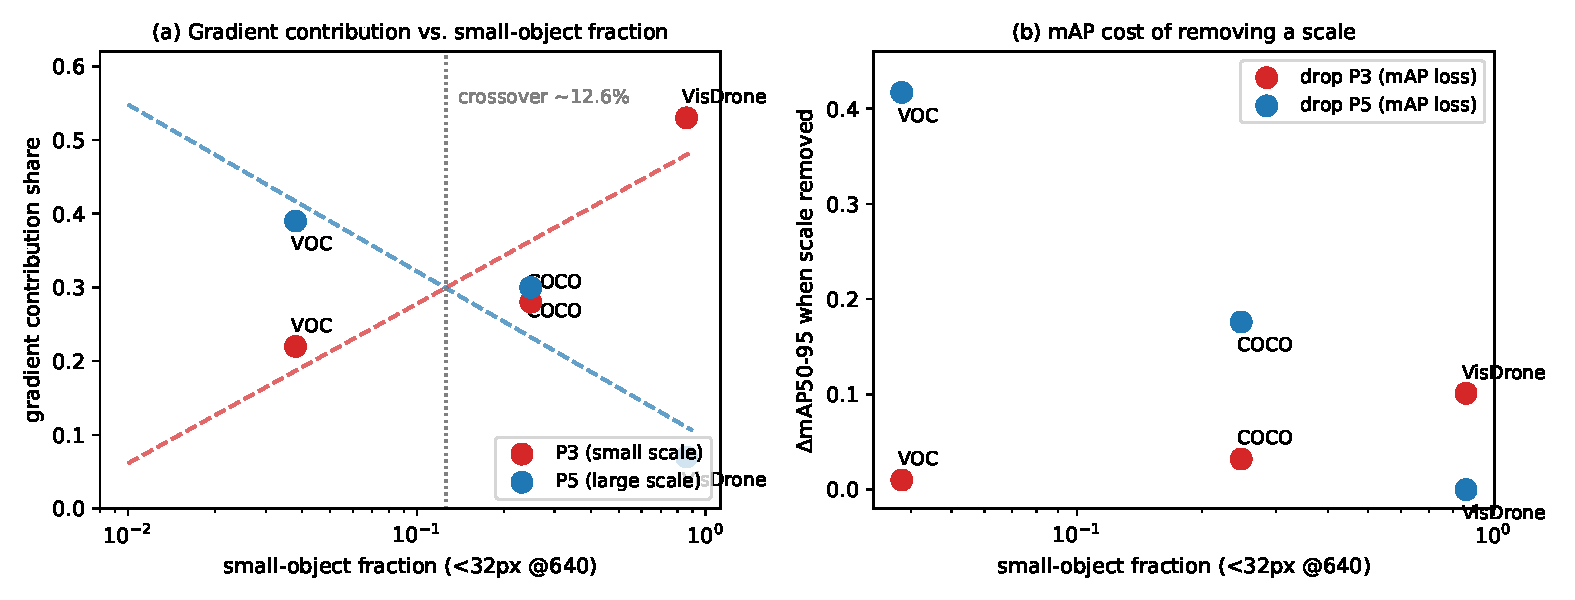
\includegraphics[width=\textwidth]{../figures/size_redundancy.pdf}
\caption{Gradient contribution (a) and mAP cost of scale removal (b) versus small-object fraction; the P3/P5 ranking reverses in our three-point trend.}
\label{fig:size}
\end{figure*}

\subsection{RQ2: cell-level redundancy is a mask-level oracle}
Cell occupancy (cells containing object centers) is 0.05/0.19/0.74\% (VOC) and 1.02/3.52/10.56\% (VisDrone) for P3/P4/P5, yet an oracle that keeps the top-5\% cells by head score retains essentially all mAP on both datasets (Table~\ref{tab:budget}). This is a mask-level analysis: it suppresses scores without saving compute. Two observations explain why detection is this sparse. First, object centers cover a tiny fraction of the grid, and NMS only needs the few cells that vote for each object, so a score-based ranker needs almost no cells to reproduce the full output. Second, gate quality matters more than cell selection alone: a ground-truth gate that keeps only cells containing object centers reaches only 0.440/0.526 mAP at 10\%/25\% budget on VOC (supplementary material), well below the self-distilled gate (0.585/0.588), because detections require the score pattern around an object, not just its center cell.
\begin{table}[h]\centering\footnotesize
\caption{Budget curves (mAP50-95, mask-level): an oracle ranking cells by the model's own head scores retains essentially all mAP at 5\% of cells; the self-distilled gate is within 0.5\,pp of full accuracy at 10\% budget (VOC: 0.5852 vs.\ 0.5899; VisDrone: 0.1719 vs.\ 0.1725) and 1.1\,pp at 5\%; the energy gate degrades much more on dense VisDrone. Full 5--75\% curves and YOLO26s/26m ablations are in the supplementary material; these numbers assume full features (real skipping: Table~\ref{tab:blockskip}).}
\label{tab:budget}
\resizebox{\linewidth}{!}{%
\begin{tabular}{lcccccc}
\toprule
 & \multicolumn{3}{c}{VOC} & \multicolumn{3}{c}{VisDrone}\\
\cmidrule(lr){2-4}\cmidrule(lr){5-7}
Budget (\% cells) & Oracle & Energy & \textbf{Distilled} & Oracle & Energy & \textbf{Distilled}\\
\midrule
5\% & 0.5895 & 0.171 & 0.5789 & 0.1725 & 0.075 & 0.1675\\
10\% & 0.5896 & 0.298 & \textbf{0.5852} & 0.1725 & 0.109 & \textbf{0.1719}\\
25\% & 0.5896 & 0.485 & 0.5882 & 0.1725 & 0.148 & 0.1724\\
\bottomrule
\end{tabular}}

\end{table}

\subsection{RQ3: FLOPs $\neq$ FPS on GPU}
The detect head is 17.3\% of total FLOPs (0.90 of 5.21~G), and preprocessing+postprocessing account for 41\% of end-to-end latency at batch 32 (batch-1 model latency 9.4~ms). We implemented real block-skipping of pruned cells (halo-padded gather $\to$ head convs $\to$ scatter); batch-32 throughput is flat or lower at every budget, so the FLOPs saved never materialize as speed (Table~\ref{tab:blockskip}):
\begin{table}[h]\centering\footnotesize
\caption{Head-level block skipping neither accelerates inference nor preserves accuracy: halo padding inflates compute and gather/scatter overhead cancels the FLOPs savings (throughput is flat or lower at every budget, 995$\to$991/986/962/911 FPS), and even the halo-only 100\%-budget variant is 19\% slower (805 FPS). The accuracy gap to the mask-level oracle (Table~\ref{tab:budget}) reflects the head seeing pruned features that differ from the full features used to train the gate.}
\label{tab:blockskip}
\resizebox{\linewidth}{!}{%
\begin{tabular}{lccc}
\toprule
Config & mAP50-95 & GFLOPs & b32 FPS\\
\midrule
Full & 0.5899 & 5.21 & 995\\
Block-skip 5\% & 0.381 & 4.79 & 991\\
Block-skip 10\% & 0.421 & 4.83 & 986\\
Block-skip 25\% & 0.478 & 4.94 & 962\\
Block-skip 50\% & 0.513 & 5.12 & 911\\
Block-skip 100\% (halo only) & 0.520 & 5.50 & 805\\
\bottomrule
\end{tabular}}
\end{table}

\subsection{Zero-training scale drop}
\begin{table}[h]\centering\footnotesize
\caption{Zero-training scale drop keeps mAP identical where the scale is redundant while cutting FLOPs/params and single-image latency; 30-epoch fine-tuning did not improve over transfer-only (0.169 vs.\ 0.173). P3-drop removes only the P3 head, whereas P5-drop also removes the P5 neck branch (Fig.~\ref{fig:scaledrop}), which is why the savings differ.}
\label{tab:scaledrop}
\resizebox{\linewidth}{!}{%
\begin{tabular}{lccccc}
\toprule
 & mAP50-95 & GFLOPs & Params(M) & b1 latency (ms) & b1 FPS\\
\midrule
\multicolumn{6}{l}{\emph{VOC: drop P3 (head-only, zero training)}}\\
Full & 0.5899 & 5.21 & 2.38 & 9.42 & 106\\
P3-drop & 0.5806 & 4.93 & 2.36 & 8.43 & 119\\
\multicolumn{6}{l}{\emph{VisDrone: drop P5 (zero training)}}\\
Full & 0.1725 & 5.20 & 2.38 & 10.02 & 100\\
\textbf{P5-drop} & \textbf{0.1725} & \textbf{4.66} & \textbf{1.70} & \textbf{9.40} & \textbf{106}\\
\bottomrule
\end{tabular}}

\end{table}
\begin{table}[h]\centering\footnotesize
\caption{Scale drop vs.\ input-resolution scaling. On VisDrone (85.9\% objects $<$32\,px), resolution scaling loses 2.8--3.5\,pp because it destroys small-object detail, while P5-drop keeps mAP identical and cuts latency by 6\%; on VOC, where small objects are rare, resolution scaling is cheaper.}
\label{tab:rescomp}
\resizebox{\linewidth}{!}{%
\begin{tabular}{lcccc}
\toprule
 & mAP50-95 & GFLOPs & b32 FPS & b1 latency (ms)\\
\midrule
\multicolumn{5}{l}{\emph{VOC (small-object fraction 3.8\%)}}\\
Full @640 & 0.5899 & 5.21 & 603 & 9.42\\
Full @512 & 0.5759 & --- & 1033 & ---\\
Full @480 & 0.5710 & --- & 1114 & ---\\
P3-drop @640 & 0.5806 & 4.93 & 769 & 8.43\\
\multicolumn{5}{l}{\emph{VisDrone (small-object fraction 85.9\%)}}\\
Full @640 & 0.1725 & 5.20 & 634 & 10.02\\
Full @512 & 0.1450 & --- & 910 & ---\\
Full @480 & 0.1378 & --- & 1009 & ---\\
\textbf{P5-drop @640} & \textbf{0.1725} & \textbf{4.66} & \textbf{670} & \textbf{9.40}\\
\bottomrule
\end{tabular}}

\end{table}

We do not pursue difficulty routing or early exit as speed-ups (Sec.~5).

\section{Negative results and lessons}
Backbone early exit is infeasible on VOC: detection from P3-only or P3+P4 features yields 0.022/0.159 mAP, because deep features are the detection representation itself. Head-level token skipping does not accelerate GPUs (Table~\ref{tab:blockskip}), a cautionary result for FLOPs-only claims~\cite{rao2021dynamicvit,liang2022evit}; even the halo-only variant that skips no cells is 19\% slower than the baseline, so the gather/scatter and halo-padding overhead alone exceeds any possible saving in this head. Fine-tuning a redundant-scale drop can also hurt (0.169 vs.\ 0.173).

\section{Discussion}
Why is scale redundancy data-dependent? In a feature pyramid, the small-object scale P3 operates at the highest resolution and carries the fine detail that small objects need, while the deep scale P5 carries the most semantic, lowest-resolution features. When a dataset is dominated by large objects (VOC, 3.8\% small), the high-resolution P3 features are barely used by the head and can be dropped with almost no loss; when it is dominated by small objects (VisDrone, 85.9\% small), P3 is the critical scale and the redundant one is instead P5. The gradient contributions in Table~\ref{tab:scales} reflect exactly this allocation of the loss to scales, which is why the small-object fraction $s$ is a usable (if imperfect) predictor of the redundant scale. The three-point fit should therefore be read as a diagnostic trend for a given architecture, not as a universal law: other architectures that allocate gradients differently (e.g., transformer-based necks) may shift the crossover.

The negative results also carry a general lesson for efficiency research on CNN detectors. Head-level token pruning reports FLOPs savings that do not transfer to GPU throughput, because dense convolutions cannot skip arbitrary cells without gather/scatter overhead and halo padding; attention models, by contrast, prune tokens natively. Reporting latency (batch-1 and batch-32) alongside FLOPs, as we do, is therefore essential, and we hope the community adopts latency reporting as a default in detector efficiency papers.

Finally, the zero-training recipe is deliberately conservative: it only removes a scale when the data already shows it is redundant, so no accuracy is traded for speed. This distinguishes it from retraining-based pruning~\cite{yan2023mccp,han2015pruning}, which can remove more compute at the cost of an optimization loop; the two are complementary, and the scale drop can be composed with channel pruning as a first, training-free step.

\section{Conclusion}
Detectors do over-see, but where the redundancy lives is dictated by the data. Across VOC, COCO, and VisDrone, the redundant scale is dataset-dependent---P3 is nearly redundant on VOC and critical on VisDrone, while P5 is completely redundant on VisDrone---and gradient contributions track the small-object fraction, with the P3/P5 ranking reversing between 3.8\% and 24.8\% small objects (a three-point trend, not a law). Cell-level redundancy is large but, in our measurements, only a mask-level oracle: real block skipping neither speeds up GPU inference nor preserves accuracy without re-training. Where a scale is truly redundant, dropping it is zero-training and cuts single-image latency by 6--12\% at identical mAP---the right choice where the cheap generic alternative fails: on dense small-object data (VisDrone), resolution scaling loses 2.8--3.5\,pp while P5-drop loses nothing.

Equally important is what does not work: backbone early exit is infeasible, and fine-tuning a redundant-scale drop can hurt. These negative results argue for dataset-aware efficiency and for reporting latency, not just FLOPs. Limitations include three datasets and models up to YOLO26m (plus a YOLO11n architecture check); the $\ln s$ trend and the 12.6\% crossover are empirical fits that must be re-validated on remote sensing, medical, or industrial data. Edge-deployment latency (Jetson/TensorRT or mobile SoCs) is explicitly out of scope: all latency numbers are desktop-GPU (RTX 5070), and measuring the zero-training recipe on real edge hardware is left to future work.

From a practitioner's perspective the recipe is simple: estimate the small-object fraction of the target data, use the fitted trend (or a single scale-removal probe) to identify the least important scale, remove it, and reuse the remaining weights without training. Because the ranking is stable across model sizes and architectures (Table~\ref{tab:robust}), the decision transfers between YOLO variants on the same data. We leave three extensions to future work: (i) validating the $\ln s$ trend on more diverse distributions, such as remote sensing, medical imaging, and industrial inspection, where the small-object fraction can exceed 95\% or drop below 1\%; (ii) measuring the zero-training recipe on edge hardware (Jetson/TensorRT), where batch-1 latency and power matter more than desktop throughput; and (iii) extending the per-scale analysis to transformer-based detectors such as RT-DETR, whose token-based computation may make the mask-level oracle exploitable in practice.

\section*{CRediT authorship contribution statement}
\textbf{Yuanchao Yan}: Conceptualization, Methodology, Software, Validation, Writing -- original draft. \textbf{Xin Yan}: Investigation, Data curation, Validation. \textbf{Jianlong Liu}: Writing -- review \& editing, Supervision.

\section*{Declaration of competing interest}
The authors declare that they have no known competing financial interests or personal relationships that could have appeared to influence the work reported in this paper.

\section*{Data availability}
All datasets used in this study (PASCAL VOC, MS COCO, and VisDrone) are publicly available from their official sources. Code and models are available at \url{https://github.com/Noisercontrollers/yolo-scale-drop}.

\bibliographystyle{model2-names}
\bibliography{../refs}

\end{document}
